
\chapter{Test auf realem Roboter}
\authorsection{\editortobias}

% \begin{itemize}
% 	\item Test auf realem Roboter erst spät möglich
% 	\item Schwer einzelne Komponenten zu testen da es viele Abhängigkeiten gibt
% 	\item Insbesondere der Steuerungs/Bahnplanungs/Hindernis Teil ist sowohl von den Laserscannern als auch vom Kinect-Teil abhängig.
% \end{itemize}


Nachdem die Ergebnisse der verschiedenen Gruppen in den Haupt-Entwicklungsstrang integriert sind, kann nach mehrmonatigem Testen in der Simulation mit Tests auf der realen Roboterplattform begonnen werden.

Ein Test mit \gls{hollie} zu einem früheren Zeitpunkt ist aufgrund der Abhängigkeiten zwischen den Komponenten nicht möglich.
Insbesondere das \lstinline{SegwayOmniBehaviours}-Modul, welches die Steuerung, Bahnplanung, sowie Kollisionsvermeidung übernimmt, ist beispielsweise sowohl von der Lokalisierung als auch von der Kinect abhängig.

Im Folgenden werden die Testumgebung sowie die während der Testphase aufgetretenen Schwierigkeiten beschrieben.


\section{Testumgebung}
\authorsection{\editortobias}

% \begin{itemize}
% 	\item Aufgebaute Umgebung
% 	\begin{itemize}
% 		\item FZI, oberes Stockwerk
% 		\item erste Tests in Bereich ohne Hindernisse
% 		\item Abgegrenzter Bereich zur Simulation einer Büroumgebung (Siehe Motivation!)
% 		\item Karte erstellen zur Lokalisierung
% 	\end{itemize}
% 	\item Geplantes Bewegungs-Szenario
% \end{itemize}

Als Testumgebung dient das Obergeschoss im Gebäude des \gls{fzi}.
Erste Test werden in einem weitläufigen Bereich ohne Hindernisse durchgeführt.\todoprivate{Foto?}

Für weitergehende Tests (Lokalisierug, Hindernis-Umfahrung etc.) wird ein abgegrenzter Bereich zur Simulation einer Büroumgebung eingerichtet.
Dazu werden zwei fest stehende Objekte auf einer rechtwinkligen Fläche platziert, die im entsprechenden Kartenmaterial ebenfalls verzeichnet sind, s. Abb \ref{fig:map_fzi}.
Als Hindernis dient eine einfach Plastik-Mülltonne.

\begin{figure}[h]
	\centering
	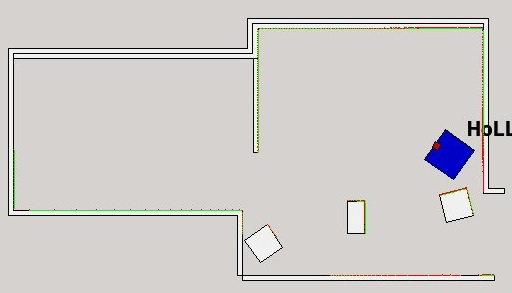
\includegraphics[width=0.6\textwidth]{graphics/map_fzi}
	\caption{Simulierte Büroumgebung für weitere Tests}
	\label{fig:map_fzi}
\end{figure}

In dieser Umgebung soll der Roboter folgendes Szenario erfüllen können:
\begin{enumerate}
  \item Person folgen ohne Hindernis
  \item Rückfahrt zum Start ohne Hindernis
  \item Pfad abfahren mit Hindernis
\end{enumerate}



\section{Aufgetretene Schwierigkeiten}
\authorsection{\editortobias}
\todo[inline]{Tobias: Schreiben}

\subsection{Laserscanner}
\label{test_schwierigkeiten_laserscanner_sec}

Der Test der auf \gls{hollie} montierten Laserscanner gestaltet sich zu Beginn nicht sehr erfolgreich.
Die zwei aufgetretenen Probleme werden im Folgenden erläutert.

\subsubsection{\glqq Unsichtbare Wand\grqq}

Das erste \emph{Problem} wird von den Praktikumsteilnehmern gerne als \glqq unsichtbare Wand\grqq\ bezeichnet.
Hintergrund dieser Namensschöpfung ist, dass sich die Scanner-Daten zwar auslesen und auch in der Benutzeroberfläche (\lstinline{mcagui}) anzeigen lassen, jedoch befindet sich in ca. $4m$ Entfernung ein großes, nur sehr leicht gekrümmtes Objekt, was von einem der beiden Scanner erkannt wird.
Auf dem Scanner-Bild (s. Abb. \ref{fig:scanner_problem}) erscheint diese Linie wie eine Wand.
Leider ist in der Realität an dieser Stelle keine Wand, sondern lediglich freier Raum.

\begin{figure}[h]
	\centering
	%\includegraphics[width=0.7\textwidth]{graphics/scanner_problem}
	\missingfigure{Sensorbild aus McaGui}
	\caption{Problem der \glqq unsichtbaren Wand\grqq\ im Scanner-Bild}
	\label{fig:scanner_problem}
\end{figure}

Die \emph{Ursache} dieser Erscheinung ist die Montage des Laserscanners am Roboter.
Da dieser nicht exakt waagerecht an \gls{hollie} angebracht ist, verläuft die Scan-Ebene nicht exakt parallel zum Untergrund.
Daher erreicht ca. die Hälfte der Scanner-Strahlen in einiger Entfernung den Boden, anstatt parallel zum Boden weiter zu verlaufen.
In der grafischen Darstellung der Messpunkte ähnelt dies dann einer Wand, da die Strahlen den Boden alle in nahezu der gleichen Entfernung treffen.

Nach Klärung der Ursache der \glqq unsichtbaren Wand\grqq\ erscheint das Problem für die weiteren Tests nicht relevant, da eine Sichweite der Laserscanner von $4m$ ausreichend ist.
Eine \emph{Lösung} ist daher nicht nötig.


\subsubsection{\glqq Tote Pixel\grqq}

Die zweite \emph{Problematik} im Zusammenhang mit den Laserscannern sind einige scheinbar \glqq tote Pixel\grqq.
Dies sind Scan-Punkte, die anhand der grafischen Darstellung offensichtlich einen Gegenstand sehr nahe an oder sogar innerhalb der Laserscanner zurückgeben.
Dieses Problem tritt bei beiden Scannern auf, und betrifft einen geringen Bruchteil der Scanner-Strahlen\todoprivate{screenshot?}.
Schwierig für \gls{hollie} ist dies deshalb, da der Roboter quasi immer in einem Hindernis steht.
Somit ist es dem A*-Algorithmus (s. Abs. \ref{kollisionsvermeidung_subsec}, S. \pageref{kollisionsvermeidung_subsec} f.) nicht möglich, eine Trajektorie um das Hindernis zu planen.
Als Folge dessen, bleibt \gls{hollie} auf der Stelle stehen, und bewegt sich nicht.

Die \emph{Ursache} dieses Problems liegt in einer unglücklich gewählten Behandlung für Scan-Punkte, die eine Fehlmessung zurückgeben.
Diese Punkte werden bis dato mit dem Wert 0 belegt.
Da dies einen Gegenstand in der Entfernung 0 bedeutet, liegen diese Scan-Punkte wie vermutet tatsächlich innerhalb der Laserscanner.

Ein erster \emph{Lösung}sversuch, gewisse Scan-Punkte für die weiteren Berechnungen einfach zu ignorieren, scheitert an der Tatsache, dass nicht immer exakt die gleichen \glqq toten Pixel\grqq\ auftreten.
Da allerdings die angesprochene Belegung mit dem Wert 0 nicht bereits in der Laserscanner-Software, sondern innerhalb der Scanner-Library auf \gls{hollie} geschieht, ist dies die Stelle, an welcher das Problem behoben werden kann:
Anstatt dem Wert 0 werden nun Fehlmessungen mit einem hinreichend großen Wert belegt, sodass die Scan-Strahlen mit Fehlmessungen nun in weiter Entfernung vom Roboter liegen.
Die \glqq toten Pixel\grqq\ bereiten damit keine Schwierigkeiten mehr.


%\begin{itemize}
%	\item \glqq Unsichtbare Wand\grqq\ in ca. 4m Entfernung
%	\begin{itemize}
%		\item Scanner nicht exakt waagerecht angebracht
%		\item nicht relevant, da Entfernung von 4m ausreichend
%	\end{itemize}
%	\item \glqq Tote Pixel\grqq\
%	\begin{itemize}
%		\item Fehlmessungen werden mit Wert 0 und nicht MAX belegt
%		\item Roboter steht immer im Hindernis -> keine Fortbewegung
%		\item Optionale Zuschaltung der Module per XML
%	\end{itemize}
%\end{itemize}



\subsection{Stromversorgung}

Ein weiteres Problem, welches beim ersten Test mit der realen Roboterplattform auftritt, ist die Stromversorgung.
Die Akkus, die auf \gls{hollie} verbaut sind, sind derzeit nicht in der Lage, sowohl den Roboter selbst als auch die darauf montierte Kinect-Kamera (s. Abs. \ref{kinect_grundlagen_sec}, S. \pageref{kinect_grundlagen_sec} ff.) mit genügend Strom zu versorgen.
Dies äußert sich darin, dass die Kinect sich im Akku-Betrieb nicht in Betrieb nehmen lässt.

Daher ist es notwendig, ein externes Netzgerät zu verwenden, und den Roboter damit mit zusätzlichem Strom zu versorgen.
Dies hat allerdings zur Folge, dass die Reichweite von \gls{hollie} durch die Länge des Kabels (ca. $5m$) zwischen Roboter und externem Netzgerät beschränkt ist.

Für die Zwecke des Praktikums ist diese Reichweite mit wenigen Einschränkungen ausreichend.

%\begin{itemize}
%	\item Robotereigene Stromversorgung reicht nicht aus für Roboter + Kinect
%	\item Netzgerät nötig
%	\item Einschränkung der Reichweite
%\end{itemize}



\subsection{Kinect}

Nach ersten Erfolgen mit dem realen Roboter stellt sich heraus, dass die Kinect-Kamera (s. Abs. \ref{kinect_grundlagen_sec}, S. \pageref{kinect_grundlagen_sec} ff.) \emph{Schwierigkeiten} damit hat, selbst bewegt zu werden und gleichzeitig auch noch einen sich wiederum auch bewegenden Menschen zu tracken.
Wenn \gls{hollie} sich zügig durch den Raum bewegt, kommt es häufig zu einem Verlust des getrackten Menschen.
Oft kommt es auch vor, dass statt des Menschen beispielsweise Säulen im Raum, Fenster, oder ähnliches als Menschen erkannt werden.
Dieses Phänomen zeigt sich auch bei rein rotatorischen Bewegungen.

Andere wissenschaftliche Mitarbeiter am \gls{fzi} haben bereits ähnliche Beobachtungen mit der Kinect gemacht.
Die \emph{Ursache} dafür liegt wohl darin, dass die Kinect ursprünglich als Einheit für den stationären Einsatz entwickelt wurde.
\Dh die Kamera steht üblicherweise fest auf einem Tisch \oae, und lediglich der Mensch vor der Kamera bewegt sich.
Im vorliegenden Fall einer sich bewegenden Kinect bewegt sich ja aus Sicht der Kamera nahezu alles im Sichtfeld (dazu gehören neben dem Menschen auch sämtliche Hintergrundobjekte etc.)
Dies scheint eine fehlerfreie Fokussierung des Menschen sehr zu limitieren.

Da eine \emph{Lösung} dieses Problems außerhalb der Möglichkeiten der Praktikumsteilnehmer liegt, wird ein \glqq work-around\grqq\ eingesetzt:
Die Geschwindigkeiten, mit denen sich \gls{hollie} fortbewegt, werden auf niedrigere Werte beschränkt.
Dazu gehören sowohl die translatorischen als auch die rotatorischen Geschwindigkeiten.
Dadurch kann die beschriebene Problematik zwar nicht endgültig beseitigt werden, die Häufigkeit des Auftretens wird jedoch reduziert.

%\begin{itemize}
%	\item verliert getrackten Menschen bei zu schneller Bewegung (insbesondere Rotation)
%	\item Verringerung der Geschwindigkeit (Rotation sowie Translation)
%\end{itemize}


\subsection{Weitere Probleme}

\begin{itemize}
	\item Odometrie auf Teppichboden
	\item SW-Bugs
	\item \ldots
\end{itemize}




